\documentclass{article}
\usepackage{a4wide}
\usepackage[utf8]{inputenc}
\usepackage{amsmath}
\usepackage{mathtools}
\usepackage{amssymb}
\usepackage[english]{babel}
\usepackage{mdframed}
\usepackage{systeme,}
\usepackage{lipsum}
\usepackage{relsize}
\usepackage{caption}
\usepackage{tikz}
\usetikzlibrary{shapes.geometric}
\usepackage{tikz-3dplot}
\usepackage{pgfplots}
\usepackage{harpoon}%
\usepackage{graphicx}
\usepackage{wrapfig}
\usepackage{subcaption}
\usepackage{authblk}
\usepackage{float}
\usepackage{listings}
\usepackage{xcolor}
\usepackage{amsmath}
\usepackage{chngcntr}
\usepackage{amsthm}
\usepackage{comment}
\usepackage{commath}
\usepackage{hyperref}%Might remove, adds link to each reference
\usepackage{url}
\usepackage{calligra}


\newcommand{\w}{\omega}
\newcommand{\curl}[1]{\mathbf{\nabla}\times \mathbf{#1}}
\newcommand{\grad}{\mathbf{\nabla}}
\newcommand{\dive}[1]{\mathbf{\nabla}\cdot \mathbf{#1}}
%\newcommand{\crr}{\mathfrak{r}}



\DeclareMathAlphabet{\mathcalligra}{T1}{calligra}{m}{n}
\DeclareFontShape{T1}{calligra}{m}{n}{<->s*[2.2]callig15}{}
\newcommand{\crr}{\mathcalligra{r}\,}
\newcommand{\boldscriptr}{\pmb{\mathcalligra{r}}\,}
\newcommand{\res}[2]{\text{Res}(#1,#2)}
\newcommand{\laplace}{\nabla^2}
\newcommand{\trace}{\text{Tr}}

\title{Handin3}
\author{Author : Andreas Evensen}
\date{Date: \today}
\definecolor{codegreen}{rgb}{0,0.6,0}
\definecolor{codegray}{rgb}{0.5,0.5,0.5}
\definecolor{codepurple}{rgb}{0.58,0,0.82}
\definecolor{backcolour}{rgb}{0.95,0.95,0.92}

\lstdefinestyle{mystyle}{
    backgroundcolor=\color{backcolour},   
    commentstyle=\color{codegreen},
    keywordstyle=\color{magenta},
    numberstyle=\tiny\color{codegray},
    stringstyle=\color{codepurple},
    basicstyle=\ttfamily\footnotesize,
    breakatwhitespace=false,         
    breaklines=true,                 
    captionpos=b,                    
    keepspaces=true,                 
    numbers=left,                    
    numbersep=5pt,                  
    showspaces=false,                
    showstringspaces=false,
    showtabs=false,                  
    tabsize=2
}

\lstset{style=mystyle}

\begin{document}

\maketitle
\section{Biharmonic equation}
Consider the Navier-Cauchy equation in the absence of anybody forces - the only forces are at boundaries
\begin{align}
    (1-2\sigma)\laplace\mathbf{u} + \nabla\left(\nabla\cdot \mathbf{u}\right) = 0,\label{eq:navier-cauchy}
\end{align}where $\mathbf{u}$ is the deformation field. Show that $\mathbf{u}$ satisfies the bi-harmonic equation
\begin{align*}
    \nabla^4\mathbf{u} = 0,
\end{align*}even if there is a constant gravitational force acting on the body. It is useful to remember that although
$\mathbf{u}$ may satisfy a biharmonic equation any solution of the biharmonic equation is not a solution of the Navier-Cauchy equation.
Now show that if $\mathbf{v}$ is a solution of the biharmonic equation then a general solution for the Navier-Cauchy equation (without volume force) can be written as
\begin{align*}
    \mathbf{u} = \laplace\mathbf{v} -\frac{1}{2(1-\sigma)}\nabla\left(\nabla\cdot\mathbf{u}\right).
\end{align*}
\subsection*{\textit{Hint}}
Assume $\mathbf{u}$ is on the form
\begin{align*}
    \mathbf{u} = \laplace\mathbf{v}+ A\nabla\left(\nabla\cdot\mathbf{v}\right),
\end{align*}where $\mathbf{v}$ solves the bi-harmonic equation. Then substitute this $\mathbf{u}$ into the Navier-Cauchy equation (without volume force) to find A.
\subsection*{Answer}
We first show that $\mathbf{u}$ satisfies the bi-harmonic equation. We start by taking the divergence of the Navier-Cauchy equation:
\begin{align*}
    0 &= \nabla\cdot\left((1-2\sigma)\laplace\mathbf{u} + \nabla\left[\nabla\cdot \mathbf{u}\right]\right)\\
    &= (1-2\sigma)\laplace\left[\nabla\cdot\mathbf{u}\right] + \nabla\cdot\left(\nabla\left[\nabla\cdot \mathbf{u}\right]\right)\\
    &= (1-2\sigma)\laplace\left[\nabla\cdot\mathbf{u}\right] + \nabla\cdot\left(\laplace\mathbf{u}\right)\\
    \implies& \laplace\left[\nabla\cdot\mathbf{u}\right] = 0.
\end{align*}Taking the Laplacian operator of the Navier-Cauchy equations yields:
\begin{align*}
    0 &= \laplace\left[(1-2\sigma)\laplace\mathbf{u} + \nabla\left(\nabla\cdot \mathbf{u}\right)\right]\\
    &= (1-2\sigma)\laplace\laplace\mathbf{u} + \laplace\left[\nabla\left(\nabla\cdot \mathbf{u}\right)\right]\\
    &= (1-2\sigma)\nabla\cdot\laplace\left[\nabla\cdot\mathbf{u}\right] + \left(\nabla^4\left[\mathbf{u}\right]\right)\\
    &= \nabla^4\mathbf{u}
\end{align*} In the case of a constant gravitational field, then we take the divergence of a constant vector field $\tilde{\mathbf{g}}$, which is zero. Thus, the biharmonic equation still holds for a constant gravitational field.
One can expand that statement and say that it holds for all vector-fields of which the divergence is zero.
Now suppose that $\mathbf{u}$ can be written as in the hint, using that $\mathbf{v}$ is a solution of the biharmonic equation, we rewrite the Navier-Cauchy equation:
\begin{align*}
    (1-2\sigma)\laplace{\mathbf{u}} &=- \nabla\left[\nabla\cdot\mathbf{u}\right]\\
    &= -\nabla\left(\nabla\cdot\left[\laplace{\mathbf{v}} + A\nabla\left(\nabla\cdot\mathbf{v}\right)\right]\right)\\
    &= -\left(\nabla^4\mathbf{v} + \nabla\cdot A\nabla(\nabla\cdot\mathbf{v})\right)\\
    &= -\nabla\cdot A\nabla(\nabla\cdot\mathbf{v}) = -A\left(\nabla\cdot\laplace\mathbf{v}\right)\\
    \implies \laplace{\mathbf{u}} &= -\frac{A}{1-2\sigma}\left(\nabla\cdot\laplace\mathbf{v}\right)
\end{align*}Using this result, one obtains the following:

\begin{align*}
    \mathbf{u} &= \laplace\mathbf{v} - \frac{1}{2(1-\sigma)}\nabla\left(\nabla\cdot\mathbf{u}\right).
\end{align*}

\section*{Question 2}
What is the equation of deformation of a small volume in a homogeneous and isotropic material in three dimensions?

\subsection*{Answer}
For an isotropic material and homogeneous material, the stress is given by:
\begin{align*}
    \sigma_{\alpha,\beta} = \frac{Y}{1+\sigma_p}\left(s_{\alpha,\beta} + \frac{\sigma_p}{1-2\sigma_p}s_{\kappa, \kappa}\delta_{\alpha,\beta}\right),
\end{align*}where $Y$ is the Young's modulus, $\sigma_p$ is the Poisson's ratio, $s_{\alpha,\beta}$ is the strain tensor, and $\delta_{\alpha,\beta}$ is the Kronecker delta.
Rewriting the stress-tensor in terms of the deformation field, we get:
\begin{align*}
    \sigma_{\alpha,\beta} &= \frac{Y}{1+\sigma_p}\left(\frac{1}{2}\left(\frac{\partial u_\alpha}{\partial x_\beta} + \frac{\partial u_\beta}{\partial x_\alpha}\right) + \frac{\sigma_p}{1-2\sigma_p}\left(\frac{\partial u_\kappa}{\partial x_\kappa}\right)\delta_{\alpha,\beta}\right)\\
    \sigma &= \frac{Y}{1 + 2\sigma_p}\left(\frac{1}{2}\left[\nabla(u) + \nabla(u)^T\right] + \frac{\sigma_p}{1-2\sigma_p}\text{tr}(\nabla u)\right)
\end{align*} In the absence of body forces, the equation of motion is given by:
\begin{align*}
    0 &= \nabla\cdot \sigma\\
    &= \frac{Y}{1 + 2\sigma_p}\nabla\cdot\left(\frac{1}{2}\left[\nabla(u) + \nabla(u)^T\right] + \frac{\sigma_p}{1-2\sigma_p}\text{tr}(\nabla u)\right)
\end{align*}
\begin{comment}
We can now write the equation of deformation of a small volume in a homogeneous and isotropic material in three dimensions:
\begin{align*}
    \frac{\partial \sigma_{\alpha,\beta}}{\partial x_\beta} &= \rho\frac{\partial^2 u_\alpha}{\partial t^2}\\
    \implies \frac{\partial}{\partial x_\beta}\left(\frac{Y}{1+\sigma}\left(\frac{1}{2}\left(\frac{\partial u_\alpha}{\partial x_\beta} + \frac{\partial u_\beta}{\partial x_\alpha}\right) + \frac{\sigma}{1-2\sigma}\left(\frac{\partial u_\kappa}{\partial x_\kappa}\right)\delta_{\alpha,\beta}\right)\right) &= \rho\frac{\partial^2 u_\alpha}{\partial t^2}\\
    \implies \frac{Y}{1+\sigma}\left(\frac{1}{2}\left(\frac{\partial^2 u_\alpha}{\partial x_\beta^2} + \frac{\partial^2 u_\beta}{\partial x_\alpha\partial x_\beta}\right) + \frac{\sigma}{1-2\sigma}\left(\frac{\partial^2 u_\kappa}{\partial x_\kappa\partial x_\beta}\right)\delta_{\alpha,\beta}\right) &= \rho\frac{\partial^2 u_\alpha}{\partial t^2}\\
    \implies \frac{Y}{1+\sigma}\left(\frac{1}{2}\left(\frac{\partial^2 u_\alpha}{\partial x_\beta^2} + \frac{\partial^2 u_\beta}{\partial x_\alpha\partial x_\beta}\right) + \frac{\sigma}{1-2\sigma}\left(\frac{\partial^2 u_\kappa}{\partial x_\kappa\partial x_\beta}\right)\delta_{\alpha,\beta}\right) &= \rho\frac{\partial^2 u_\alpha}{\partial t^2}\\
    \implies \frac{Y}{1+\sigma}\left(\frac{1}{2}\left(\frac{\partial^2 u_\alpha}{\partial x_\beta^2} + \frac{\partial^2 u_\beta}{\partial x_\alpha\partial x_\beta}\right) +
    \frac{\sigma}{1-2\sigma}\left(\frac{\partial^2 u_\alpha}{\partial x_\beta^2} + \frac{\partial^2 u_\beta}{\partial x_\alpha\partial x_\beta}\right)\right) &= \rho\frac{\partial^2 u_\alpha}{\partial t^2}\\
    \implies \frac{Y}{1+\sigma}\left(\frac{1+\sigma}{2(1-2\sigma)}\left(\frac{\partial^2 u_\alpha}{\partial x_\beta^2} + \frac{\partial^2 u_\beta}{\partial x_\alpha\partial x_\beta}\right)\right) &= \rho\frac{\partial^2 u_\alpha}{\partial t^2}\\
    \implies \frac{Y}{1+\sigma}\left(\frac{1+\sigma}{2(1-2\sigma)}\left(\frac{\partial^2 u_\alpha}{\partial x_\beta^2} + \frac{\partial^2 u_\beta}{\partial x_\alpha\partial x_\beta}\right)\right) &= \rho\frac{\partial^2 u_\alpha}{\partial t^2}\\
    \implies \frac{Y}{2(1-2\sigma)}\left(\frac{\partial^2 u_\alpha}{\partial x_\beta^2} + \frac{\partial^2 u_\beta}{\partial x_\alpha\partial x_\beta}\right) &= \rho\frac{\partial^2 u_\alpha}{\partial t^2}\\
    \implies \frac{Y}{2(1-2\sigma)}\left(\frac{\partial^2 u_\alpha}{\partial x_\beta^2} + \frac{\partial^2 u_\beta}{\partial x_\alpha\partial x_\beta}\right) &= \rho\frac{\partial^2 u_\alpha}{\partial t^2}\\
    \implies \frac{Y}{2(1-2\sigma)}\left(\frac{\partial^2 u_\alpha}{\partial x_\beta^2} + \frac{\partial^2 u_\beta}{\partial x_\alpha\partial x_\beta}\right) &= \rho\frac{\partial^2 u_\alpha}{\partial t^2}\\
\end{align*}This is the equation of deformation of a small volume in a homogeneous and isotropic material in three dimensions.
\end{comment}
\section*{Question 3}
Now consider the kind of deformation where $u_z = 0$ everywhere in a three-dimensional body (that is homogeneous and isotropic with elastic coefficients $Y$ and $\sigma_p$) and $u_x$ and $u_y$ are functions of $x$ and $y$ alone (not functions of $z$).
Note that the dimension on the body along the z direction remains constant. Hence, although $u_z = 0$ everywhere, $\sigma_{z,z}$ is not zero.
\subsection*{a)}
What is the equations of equilibrium involving the stresses $\sigma_{i,j}$ where $i,j$ are $x$ and $y$.

\subsubsection*{Answer}
In order to find the equilibrium equations involving the stresses $\sigma_{i,j}$, we need to find the stresses $\sigma_{i,j}$.
\begin{align*}
    \sigma_{x,x} &= \frac{Y}{1+\sigma_p}\left(s_{x,x} + \frac{\sigma_p}{1-2\sigma_p}s_{\kappa, \kappa}\delta_{x,x}\right)\\
    \sigma_{x,y} &= \frac{Y}{1+\sigma_p}\left(s_{x,y} + \frac{\sigma_p}{1-2\sigma_p}s_{\kappa, \kappa}\delta_{x,y}\right)\\
    &= \frac{Y}{1+\sigma_p}\left(s_{x,y}\right)\\
    \sigma_{y,x} &= \frac{Y}{1+\sigma_p}\left(s_{y,x} + \frac{\sigma}{1-2\sigma}s_{\kappa, \kappa}\delta_{y,x}\right)\\
    &= \frac{Y}{1+\sigma_p}\left(s_{y,x}\right)\\
    \sigma_{y,y} &= \frac{Y}{1+\sigma_p}\left(s_{y,y} + \frac{\sigma_p}{1-2\sigma_p}s_{\kappa, \kappa}\delta_{y,y}\right)
\end{align*}
Balancing the directions, without any body-forces:
\begin{align*}
    \text{$\hat{x}$: } \frac{\partial \sigma_{x,x}}{\partial x} + \frac{\partial \sigma_{x,y}}{\partial y} = 0\\
    \text{$\hat{y}$: } \frac{\partial \sigma_{y,y}}{\partial y} + \frac{\partial \sigma_{y,x}}{\partial x} = 0\\
\end{align*}

\subsection*{b)}
Show that for a scalar function $\psi(x,y)$ the equations of equilibrium are satisfied by the following choice
\begin{align*}
    \sigma_{x,x} = \frac{\partial^2\psi(x,y)}{\partial y^2}\\
    \sigma_{x,y} = -\frac{\partial^2\psi(x,y)}{\partial y\partial x}\\
    \sigma_{y,y} = \frac{\partial^2\psi(x,y)}{\partial x^2}
\end{align*}

\subsubsection*{Answer}
\begin{comment}
Firstly, since $\sigma_{i,j}$ can be expressed in terms of $u$, one can write the sum:
\begin{align*}
    \sigma_{x,x} + \sigma_{y,y} &= \underbrace{\frac{Y(1-2\sigma_p)}{1+\sigma_p}}_{P}\left(\frac{\partial u_x}{\partial x} + \frac{\partial u_y}{\partial y}\right)
\end{align*}This is divergence of the deformation field, which in itself is only a function of $x$ and $y$. We call that function $\psi(x,y) = \nabla\cdot\mathbf{u}$.
Taking the square derivatives of $\psi(x,y)$, one gets the following:
\begin{align*}
    \frac{\partial^2\psi(x,y)}{\partial x^2} &= P\frac{\partial^2}{\partial x^2}\left(\frac{\partial u_x}{\partial x} + \frac{\partial u_y}{\partial y}\right)\\
    &= \sigma_{y,y}\\
    \frac{\partial^2\psi(x,y)}{\partial y^2} &= P\frac{\partial^2}{\partial y^2}\left(\frac{\partial u_x}{\partial x} + \frac{\partial u_y}{\partial y}\right)\\
    &= \sigma_{x,x}\\
    \frac{\partial^2\psi(x,y)}{\partial y\partial x} &= P\frac{\partial^2}{\partial y\partial x}\left(\frac{\partial u_x}{\partial x} + \frac{\partial u_y}{\partial y}\right)\\
    &= \sigma_{x,y}
\end{align*}
\end{comment}
Suppose that there exists a function $\psi(x,y)$ such that the above equations are satisfied. Applying this to the equations of equilibrium, one gets the following:
\begin{align*}
    \frac{\partial}{\partial x}\left(\frac{\partial^2\psi}{\partial y^2}\right) + \frac{\partial}{\partial y}\left(\frac{\partial^2\psi}{\partial x\partial y}\right) &= 0\\
    \frac{\partial}{\partial y}\left(\frac{\partial^2\psi}{\partial x^2}\right) + \frac{\partial}{\partial x}\left(\frac{\partial^2\psi}{\partial x\partial y}\right) &= 0\\
    \implies \frac{\partial^3\psi}{\partial x\partial y^2} +\frac{\partial^3\psi}{\partial x\partial^2 y^2} &= 0\\
    \implies \frac{\partial^3\psi}{\partial y\partial x^2} + \frac{\partial^3\psi}{\partial x^2\partial y} &= 0
\end{align*}Since the two above conditions have to be satisfied, one finds that the Airy stress function $\psi(x,y)$ is given by:
\begin{align*}
    \psi(x,y) = \frac{1}{2}\left(\sigma_{x,x}x^2 + 2\sigma_{x,y}xy + \sigma_{y,y}y^2\right)
\end{align*}


\subsection*{c)}
Find out what kind of partial differential equation $\psi$ obeys. \textit{Hint:} Write the stress in terms of strains
\begin{align*}
    \sigma_{\alpha, \beta} = \frac{Y}{1+\sigma}\left(s_{\alpha,\beta} + \frac{\sigma}{1-2\sigma}s_{\kappa, \kappa}\delta_{\alpha,\beta}\right).
\end{align*}Take trace on both sides. The function $\psi$ is known as the Airy stress function.

\subsubsection*{Answer}
Using the hint, one gets the following:
\begin{align*}
    \trace\left(\sigma_{\alpha, \beta}\right) &= \frac{Y}{1+\sigma}\trace\left(s_{\alpha,\beta} + \frac{\sigma}{1-2\sigma}s_{\kappa, \kappa}\delta_{\alpha,\beta}\right)\\
    \sigma_{x,x} + \sigma_{y,y} + \sigma_{z,z} &= \frac{Y}{1+\sigma}\left(\trace(S) + \frac{\sigma}{1-2\sigma}\trace(S)\right)\\
    &=\frac{Y}{1+\sigma}\left(s_{x,x} + s_{y,y} + s_{z,z} + \frac{\sigma}{1-2\sigma}\left[s_{x,x} + s_{y,y} + s_{z,z}\right]\right)
\end{align*}




\section*{Contact mechanics}
A sphere made of isotropic material with Young's modulus $Y$ and Poisson's ratio $\sigma$ and mass $M$ with uniform density falls from a height $h$ on a flat surface.
The gravitational acceleration $g$ is constant. The surface is very hard compared to the sphere such that you can ignore any deformation of the surface. Estimate the amount of time the sphere stays in contact with the surface.

\subsection*{Answer}
In order to find the contact time, one needs to generalize the concepts used earlier. One states that the potential energy of the sphere is given by:
\begin{align*}
    E_p = mgh,
\end{align*}and the kinetic energy is given by:
\begin{align*}
    E_k = \frac{1}{2}mv^2.
\end{align*}At point of contact, the potential energy is zero and of the energy is kinetic energy. The velocity at that point is given by:
\begin{align*}
    v = \sqrt{2gh}.
\end{align*}We approximate the hard surface as a sphere of infinite radius and thus the effective radius becomes $\frac{1}{r} = \frac{1}{R}$.
\begin{figure}[H]
    \centering
    \begin{tikzpicture}[scale = 0.5]
        \draw (0,5) circle (1);
        \draw[->] (3,5) -- (3, 0) node[right, pos = 0.5] {$h$};
        \draw[dashed] (0,0) -- (3,0);
        \draw[dashed] (0,5) -- (3,5);
        \draw (-2,0) -- (2, 0);
        \draw[dashed] (0,0) circle (1);
        \draw (1,0) arc (0:180:1);
        \draw[<->] (0,0) -- (0,-1) node[right, pos = 0.5] {$d$};
    \end{tikzpicture}
    \caption{Illustration of the sphere falling on the surface.}
    \label{fig: task4}
\end{figure}\noindent
Using the crude figure from above, expression for the height $d$:
\begin{align*}
    d = \frac{F}{\pi aY},
\end{align*}where $z$ is the depth of the indentation, $a$ is the contact area of the sphere and the sheet, and $F$ is the force exerted on the sphere/plane. The force exerted on the sphere is given by:
\begin{align*}
    F = mg
\end{align*}and the contact area is given by:
\begin{align*}
    a = \left(\frac{rF}{\pi Y}\right)^{1/3}.
\end{align*}
The system follows the following ordinary differential equation:
\begin{align*}
    \frac{\partial d}{\partial t} &= \sqrt{2gh}\\
    \partial t&=\frac{\partial d}{\sqrt{2gh}}\\
    \implies t &= \int_0^d\frac{1}{\sqrt{2gh}}dd'\\
    &= \frac{d}{\sqrt{2gh}} = \frac{\frac{mg}{\pi aY}}{\sqrt{2gh}}\\
\end{align*}This is only the time it takes for the deformation to stop, but the contact-time is also the time it takes for the sphere to lose contact with the surface, hence the actual time is given by:
\begin{align*}
    t = \frac{2mg}{\pi aY\sqrt{2gh}} = \frac{2mg}{\pi Y\sqrt{2gh}}\left(\frac{\pi Y}{r F}\right)^{\frac{1}{3}}.
\end{align*}

\section*{Problem for extra credit}
A cylinder made of isotropic material with Young's modulus $Y$ and Poisson's ratio $\sigma$ is resting on a flat surface. Ignore the deformations of the surface.
If the cylinder has mass per unit length $m$ and uniform gravitational acceleration is $g$ calculate the area of contact. Note that we did contact of spheres in class. You need to generalize the ideas to contact of cylinder with a flat surface.

\subsection*{Answer}
\begin{figure}[H]
    \centering
    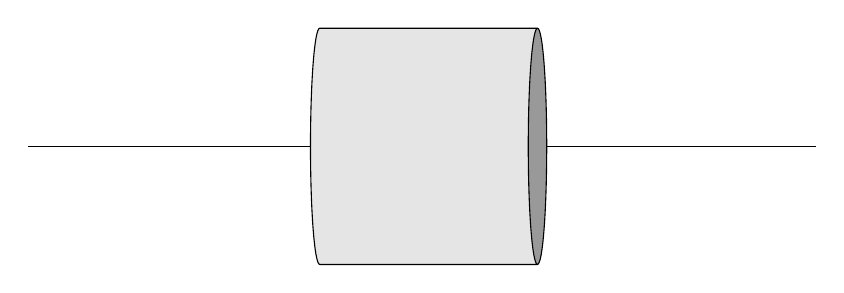
\begin{tikzpicture}
        \draw (-5,0) -- (5,0);
        \node[cylinder, 
        draw = black, 
        text = purple,
        cylinder uses custom fill, 
        cylinder body fill = black!10, 
        cylinder end fill = black!40,
        minimum size = 3cm] (c) at (0,0) {};
    \end{tikzpicture}
    \caption{Illustration of the cylinder resting on a flat surface, with some deformation}
    \label{fig: task5}
\end{figure}\noindent The contact area is in this case given by a rectangle, with width $a$ and length $L$, where $L$ is the length of the cylinder.
The area of the rectangle is given by:
\begin{align*}
    A = aL.
\end{align*}The area $A$ is a function of $a$ since it depends on the deformation of the cylinder. The height of which the cylinder is deformed is given by:
\begin{align*}
    h = u_z + \varrho^2\frac{1}{2\rho},
\end{align*}where $\rho$ is the radius of the cylinder, and $\varrho$ is the radius of the contact area. From this one finds derives the force -- distance relationship.

\end{document}
 